\documentclass{standalone}
\usepackage{tikz}
\usepackage{tkz-graph}
\usepackage{tkz-berge}

\begin{document}

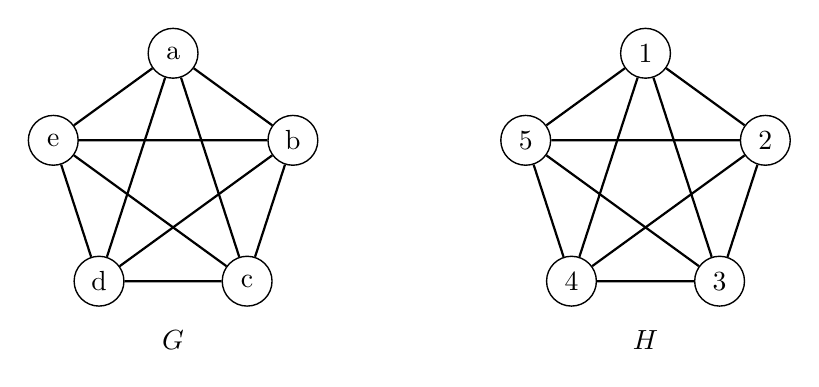
\begin{tikzpicture}
  \GraphInit[vstyle=Normal]
  \SetVertexMath
  \begin{scope}[rotate=90+(72*3)]
    \SetVertexNoLabel
    \grComplete[prefix=a,RA=1.6]{5}
    \AssignVertexLabel[]{a}{c,b,a,e,d}
  \end{scope}

  \begin{scope}[xshift=6cm, rotate=90+(72*3)]
    \SetVertexNoLabel
    \grComplete[prefix=b,RA=1.6]{5}
    \AssignVertexLabel[]{b}{3,2,1,5,4}
  \end{scope}
  \draw (0,-1.8) node [below]{$G$};
  \draw (6,-1.8) node [below]{$H$};
\end{tikzpicture}

\end{document}
